\documentclass{beamer}
\usepackage{hyperref}
\hypersetup{colorlinks,linkcolor=}
\usepackage{tikz}
\usetikzlibrary{shapes.geometric, arrows.meta, graphs}
\tikzstyle{open} = [rectangle, rounded corners, text centered, draw=black]
\tikzstyle{closed} = [rectangle, rounded corners, text centered, draw=black, fill=red!30]

\usetheme{Berlin}

\title{GLVNDized PowerVR Driver (and Zink)}
\subtitle{A least-intrusive standard-friendly solution to deliver PowerVR closed drivers on GNU/Linux desktop}
\author{Icenowy Zheng}
\institute{PLCT Lab}
\date{2025-4-30}

\begin{document}

\section{Preface}

\frame{\titlepage}

\begin{frame}
	\frametitle{PowerVR closed drivers: desktop distros' nightmare}
	The "LinuxWS" driver variant of PVR closed drivers is designed for using with Linux desktops (X11 / Wayland).
	\begin{block}{But it's problematic!}
		\begin{itemize}
			\item Problem 1: Replaces system components: Mesa, X.org, etc.
			\item Problem 2: Lacks desktop GL for most of times (desktop GL is only available for high end GPUs).
		\end{itemize}
	\end{block}
\end{frame}

\section{GLVNDizing}

\begin{frame}
	\frametitle{Refer to the Model Closed Driver}
	\begin{block}{What? A model for closed driver?}
		"Model Closed Driver" here means NVIDIA Linux Drivers. \\
		Despite of being ****ed by Linus, it's the closed GPU driver most distros packaged, and it rarely conflicts with open source drivers.
	\end{block}
	Could we make the PowerVR closed driver as harmonic with the system as NVIDIA driver?
\end{frame}

\begin{frame}
	\frametitle{Q: What does our Model do?}
	A: Make nearly every part of the driver loadable and dispatched at runtime.

	\begin{block}{Loadable entries}
		\begin{itemize}
			\item GBM: Mesa libgbm supports loads backends from \texttt{/usr/lib/gbm}.
			\item lib*GL*: NVIDIA developed \href{https://gitlab.freedesktop.org/glvnd/libglvnd}{libglvnd} for runtime loading / dispatching them.
			\item X.org server: Have loadable drivers (known as DDX) since XFree86.
		\end{itemize}
	\end{block}
\end{frame}

\begin{frame}
	\frametitle{What does Imagination do on Mesa?}
	Mesa itself is a multi-layer project, consists of a DRI implementation and a DRI loader. \\
	It implements EGL/GLX entrypoint libraries (in modern distros with GLVND, \texttt{lib\{EGL,GLX\}\_mesa.so}) via the DRI loader loading the real DRI implemenation (which does buffer management and GL(ES)). \\
	In additionit implements GBM (integrated into \texttt{libgbm.so}) via the DRI loader.
	\begin{block}{Call graph}
		\includegraphics[scale=0.53,keepaspectratio=true]{mesa_callgraph.pdf}
	\end{block}
\end{frame}

\begin{frame}
	\frametitle{What does Imagination do on Mesa?}
	The PVR closed driver contains its own DRI implementation (mostly) in \texttt{libpvr\_dri\_support.so}, only a shim for it is placed into Mesa. \\ The \texttt{libpvr\_dri\_support.so} library then dlopen's and calls \texttt{libGLESv2\_PVR\_MESA.so} to provide GLES implementation.
	\begin{block}{Call graph}
		\includegraphics[scale=0.53,keepaspectratio=true]{pvr_mesa_callgraph.pdf}
	\end{block}
\end{frame}

\begin{frame}
	\frametitle{Make Mesa loadable again}
	Modern distros are already shipping its system Mesa as GLVND loadable driver, but creating a secondary loadable Mesa isn't so easy...
	\begin{block}{Original sins of a secondary loadable Mesa}
		Not everything is made loadable in vanilla Mesa. \\
		It installs a non-loadable \texttt{libglapi.so} and provides the system \texttt{libgbm.so} with an internal ``dri'' backend.
	\end{block}
\end{frame}

\begin{frame}
	\frametitle{Make Mesa loadable again}
	\begin{block}{Solutions to \texttt{libglapi.so}}
		To make a secondary Mesa not to collide with system one, the \texttt{libglapi.so} needs to have both its name and its symbols changed.
	\end{block}
	\begin{block}{Solutions to GBM}
		The internal ``dri'' backend, in fact, is structured quite similar to a real loadable GBM backend. \\
		With a few small changes (and dropping the main libgbm code), it could be built as a loadable backend.
	\end{block}
\end{frame}

\begin{frame}
	\frametitle{From loadable to dispatched}
	The libraries are now built to be independent with system Mesa (except the GBM loader). However how could they get dispatched to?
	\begin{block}{GBM dispatching}
		The internal dri backend is considered a fallback backend in libgbm, and if \texttt{/usr/lib/gbm/\$\{DRM\_DRIVER\}\_gbm.so} exists it will be used. So just build the GBM backend as \texttt{/usr/lib/gbm/pvr\_gbm.so} and symlink to \texttt{/usr/lib/gbm/\$\{DISPLAY\_DRIVER\}\_gbm.so} and it will be picked when necessary.
	\end{block}
\end{frame}

\begin{frame}
	\frametitle{From loadable to dispatched}
	\begin{block}{EGL dispatching}
		The libglvnd library scans \texttt{/usr/share/glvnd/egl\_vendor.d} for JSON-formatted vendor driver definitions, with smaller number leads to higher priority. \\
		As the system Mesa one is \texttt{50\_mesa.json}, just name our new driver's JSON \texttt{40\_pvr.json} to let it be priortized.
	\end{block}
	\begin{block}{GLX dispatching}
		If the X server can utilize AIGLX, the GLX vendor name could be specified with ``GlxVendorLibrary'' option. \\
		However it's not the case of PowerVR closed drivers (which usually cannot do OpenGL), so ``\_\_GLX\_VENDOR\_LIBRARY\_NAME'' environment variable is used now as a hack.
	\end{block}

\end{frame}

\begin{frame}
	\frametitle{What is needed on X.org?}
	Well, theortically X.org does not need to be modified...
	\begin{block}{But what's the reality?}
		The latest X.org server release, 21.1, has quite bad GLES support in Glamor (its 2D-acceleration-on-GL implementation). \\
		In addition X.org uses some quite weird way to implement front buffer rendering with EGL -- the display buffer isn't an EGLSurface (which forces back buffer rendering), but an EGLImage as framebuffer in surfaceless mode. Some PowerVR blobs cannot handle this well and leads to display glitches.
	\end{block}
\end{frame}

\begin{frame}
	\frametitle{What is needed on X.org?}
	The X.org patches from Imagination isn't publicly available. \\
	In the development of RevyOS, I tried to reconstruct the patches by using mostly backported patches (and a few newly created ones). \\
	But, how to convert patches to a loadable modules? \\
	\begin{block}{My personal answer: xf86-video-pvrdri}
		The patches are all about the Glamor part of X.org server, which is called by the modesetting DDX (also a part of X.org server now). \\
		By extracting the modesetting DDX and glamor from the RevyOS patched X.org server, I created \href{https://github.com/Icenowy/xf86-video-pvrdri}{xf86-video-pvrdri}, a patched X.org server suitable for using with PowerVR closed drivers.
	\end{block}
\end{frame}

\begin{frame}
	\frametitle{What do we get after doing GLVNDizing?}
	\begin{block}{Gains}
		Replacing system packages is not longer needed (which makes it more safe to do system upgrades), and a newer Mesa from system could be utilized for LLVMpipe.
	\end{block}
	\begin{block}{Remaining issues}
		The closed driver is usually still GLES only, and many desktop distros are built to expect desktop GL (especially under X.org).
	\end{block}
\end{frame}

\section{Zink}

\begin{frame}
	\frametitle{Zink, twilight?}
	There is a driver inside mainline Mesa called Zink, that implements OpenGL-over-Vulkan. \\
	As PowerVR closed drivers usually come with Vulkan support, could we utilize Zink to implement desktop OpenGL? And could we just use the Zink of system Mesa?
	\begin{block}{Advertisement from Imagination}
		\begin{quote}
			Imagination GPUs now support OpenGL® 4.6 \\
			Zink is a layered OpenGL® implementation, part of the open-source Mesa project, that allows OpenGL® 4.6 content to run on top of a native Vulkan driver. For Imagination GPUs, this is a win-win.
		\end{quote}
	\end{block}
\end{frame}

\begin{frame}
	\frametitle{Zink, dream?}
	Just get a PowerVR closed driver and a Mesa 24.2 with Zink -- BOOM! Every process that calls libGL crashes!
	\begin{block}{Emergency blocklist}
		In Mesa 24.3, I added a commit to Mesa mainline that blocklisted many PowerVR closed Vulkan drivers that leads to crash, which at least allows fallback to LLVMpipe in these cases.
	\end{block}
	Investigations on mainline and patched Mesa source code shows that Zink only works on some GPUs and on PVR-patched Mesa 22.3.5, which disappoints desktop distro maintainers.
\end{frame}

\begin{frame}
	\frametitle{Background: Rogue and Volcanic}
	Open the \texttt{hwdefs} directory of a copy of PowerVR DDK kernel mode driver, two directories are shown: \texttt{rogue} and \texttt{volcanic}. \\
	This corresponds to two different GPU architectures, both listed under the name ``PowerVR'' and present in Imagination A and B series GPUs. \\
	Rogue is the legacy architecture but still used on small A/B series GPUs. The largest known Rogue is BXM-4-64. \\
	Volcanic is the new architecture for bigger GPUs, and the smallest known Volcanic is AXM-8-256.
	\begin{block}{Sidenote: GPU core naming convention since A series}
		The two numbers are just raw representation of theortical performance per clock cycle, with the former as pixels per clock and the latter as FLOPs per clock.
	\end{block}
\end{frame}

\begin{frame}
	\frametitle{Investigation on Mesa and closed Vulkan driver}
	One major visible difference between Rogue and Volcanic GPUs' closed Vulkan driver is that only Volcanic's support \texttt{deviceFeatures.geometryShader}, and the code contributed to mainline Zink blindly use geometry shaders on closed PowerVR drivers. \\
	\vfill
 	It seems that Imagination and Collabora only adapted and tested Zink on Volcanic GPUs, and Rogue ones are out of luck. \\
 	In addition, further evolution of Zink introduced more optimization and even breaked Volcanic closed driver.
\end{frame}

\begin{frame}
	\frametitle{Zink supplements, prescribed for Volcanic}
	By bisecting between 22.3 and 24.3 on a Volcanic GPU (EIC7700's AXM-8-256 used), the upstream Zink changes incompatible with the Volcanic driver could be deduced. \\
	This leads to some Mesa pull requests that adds PowerVR closed driver specific quirks to Zink (\href{https://gitlab.freedesktop.org/mesa/mesa/-/merge_requests/32342}{!32342} for not using SpV constants with arbitary types, \href{https://gitlab.freedesktop.org/mesa/mesa/-/merge_requests/32343}{!32343} for disabling descriptor buffer, \href{https://gitlab.freedesktop.org/mesa/mesa/-/merge_requests/33051}{!33051} for disabling demote SpV instruction), and finally they landed in Mesa main branch now (the first stable version containing them should be 25.2.0). \\
	These merge requests make Zink from Mesa master (or 24.0/24.3/25.0 with these patches backported) work with Volcanic closed drivers, but still not Rogue ones...
\end{frame}

\begin{frame}
	\frametitle{Zink supplements, prescribed for Rogue}
	More investigations are done on Zink on Rogue closed drivers, and it's found that their vulkan driver have some extra quirk: they require VkSubmitInfo's to have command buffers, but Zink tries to queue VkSubmitInfo's that are totally empty or have only semaphores to signal. \\
	By reverting the commit that blocklists Rogue for Zink, fixing the hardcoded assumption for using geometry shaders to do some workarounds on PowerVR closed drivers and trying to fix the problem of VkSubmitInfo's not liked by Rogue closed drivers, Zink now runs on Rogue and provides the OpenGL support that it originally lacks!
\end{frame}

\begin{frame}
	\frametitle{The holy grail of PowerVR closed driver support}
	Finally we got Zink to render (most of) a desktop on a Rogue GPU, with (Qt5) applications using desktop GL with GLX.
	\begin{center}
		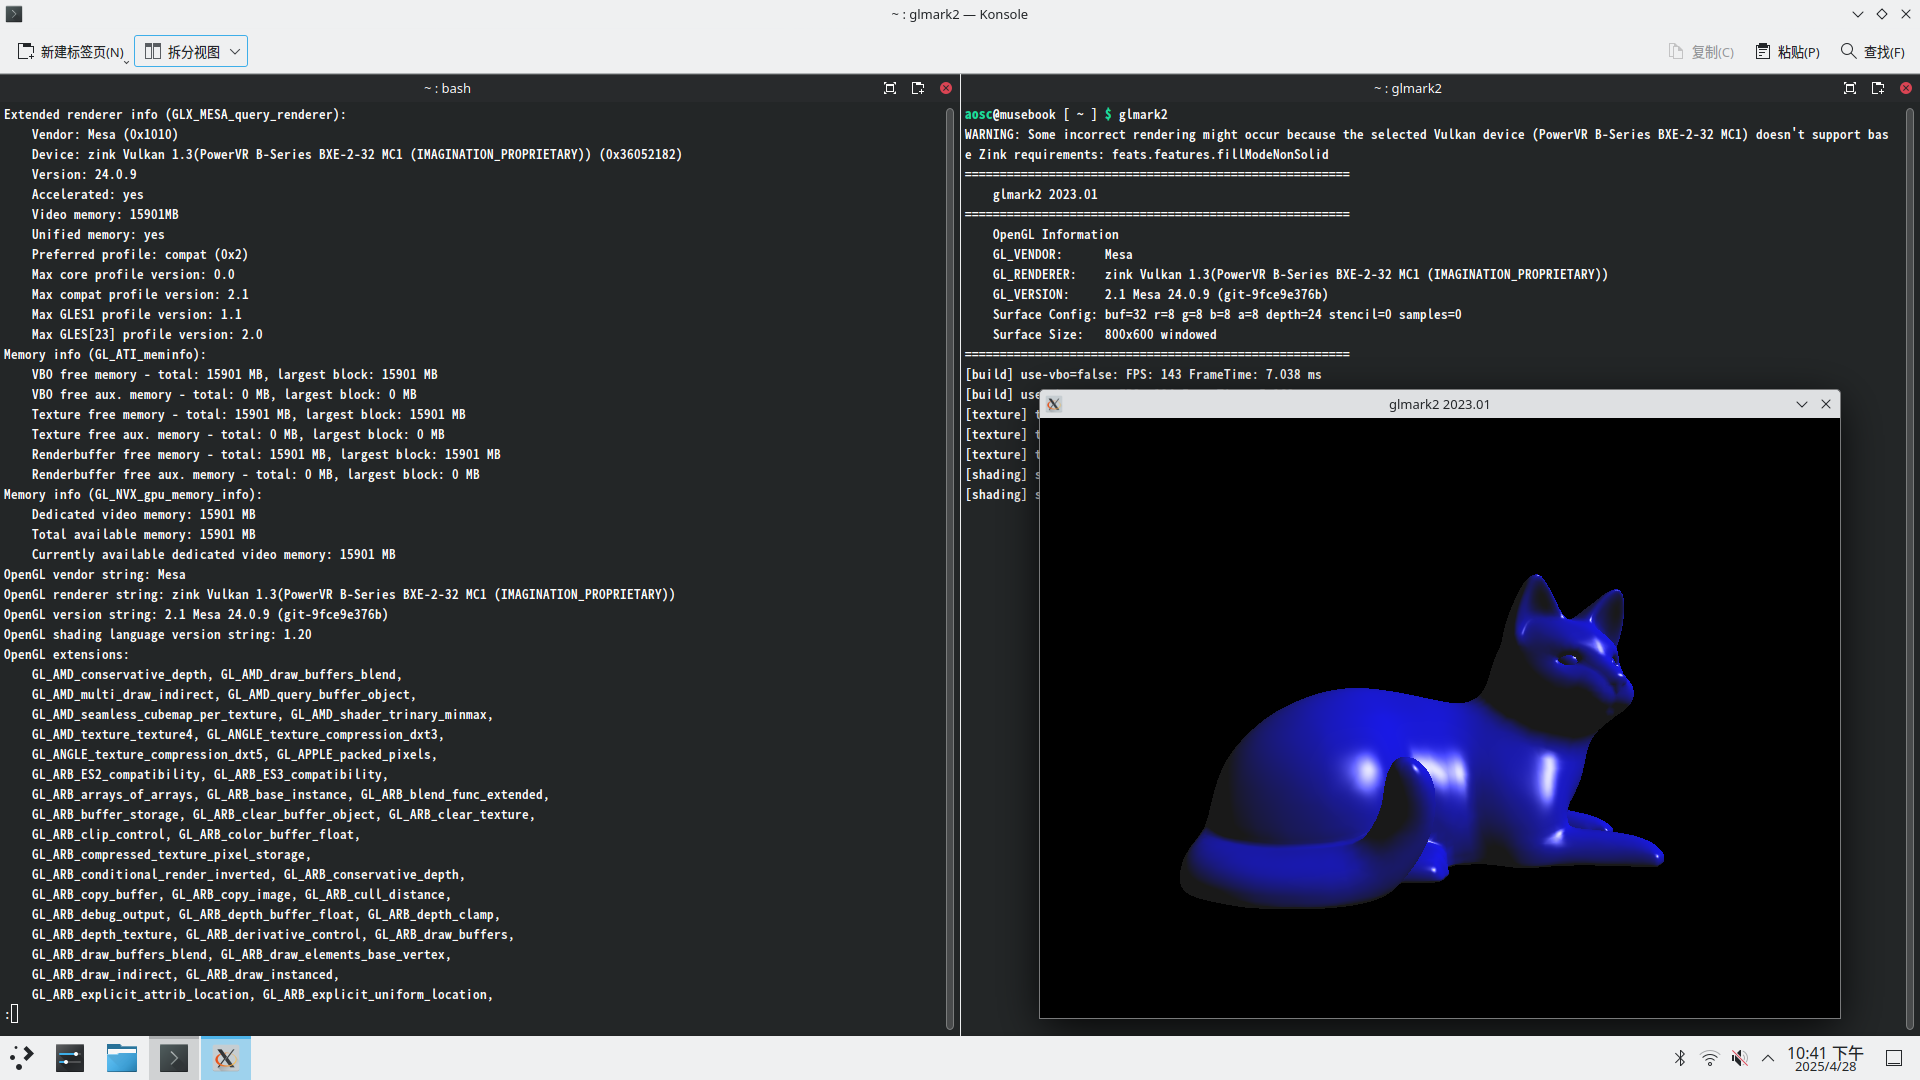
\includegraphics[scale=0.18]{rogue-zink-screenshot.png}
	\end{center}
\end{frame}

\begin{frame}
	\frametitle{Known issues and work arounds}
	Importing buffers with EGLImage still do not work with Zink on Rogue now, which prevents KWin from using Zink on Rogue. \\
	Fortunately KWin could be instructed to use GLES by setting some environment variables, and KDE's session management with Systemd makes this process easy. \\
	\begin{block}{My configuration file \texttt{/etc/systemd/user/plasma-kwin\_x11.service.d/50-force-gles.conf}}
		\texttt{[Service] \\
			Environment=KWIN\_COMPOSE=O2ES \\
			Environment=QT\_XCB\_GL\_INTEGRATION=xcb\_egl
		}
	\end{block}
\end{frame}

\begin{frame}
	\frametitle{A few further problems}
	\begin{itemize}
		\item My work to ``tidy up'' VkSubmitInfo's looks dirty (at least to me) , so I sent it only as a RFC merge request (\href{https://gitlab.freedesktop.org/mesa/mesa/-/merge_requests/34183}{!34183}), but I have gotten no comments that I requested for...
		\item Some Vulkan features (mostly related to legacy OpenGL features) are still currently required by Zink and not polyfilled (and not present in PowerVR closed drivers), which leads to a few warnings when using Zink.
		\item Of course it could be better if we can run KWin with Zink...
		\item I also explored getting rid of legacy GLES closed drivers, and failed -- the DRI implementation in Mesa seems to be not ready for renderonly devices with Zink.
	\end{itemize}
\end{frame}

\end{document}
